\documentclass{article}

\usepackage{algorithm}
\usepackage{algpseudocode}
\usepackage{amsmath}
\usepackage{amsfonts}
\usepackage{amssymb}
\usepackage{booktabs}
\usepackage{float}
\usepackage{graphicx}
\usepackage{hyperref}
\usepackage{tikz}
\usetikzlibrary{arrows.meta, positioning}


\newcommand{\indep}{\perp\!\!\!\!\perp}
\newcommand{\nindep}{\not\perp\!\!\!\!\perp}
\newcommand{\x}{\mathbf{x}}
\newcommand{\X}{\mathbf{X}}
\newcommand{\ub}{\mathbf{u}}
\newcommand{\z}{\textbf{z}}
\newcommand{\zc}{\textbf{z}_\text{causal}}
\newcommand{\C}{\mathfrak{C}}
\newcommand{\G}{\mathcal{G}}
\newcommand{\N}{\mathcal{N}}
\newcommand{\E}{\mathbb{E}}
\newcommand{\D}{\mathbb{D}}
\newcommand{\dklbar}{\,\|\,}
\newcommand{\eps}{\boldsymbol{\epsilon}}


\title{Structural Causal Models and Diffusion Probabilistic Models}
\date{Summer 2025}
\author{
	Turmanidze, Lado\\
	\texttt{turmanidze.lado@kiu.edu.ge}
	\and
	Cao, Zhuo\\
	\texttt{z.cao@fz-juelich.de}
}

\begin{document}
	
	\maketitle
	
	\begin{abstract}
	The integration of Structural Causal Models (SCMs) with Diffusion Probabilistic Models (DDPMs) presents a novel approach to enhancing causal inference and representation learning. SCMs offer a comprehensive framework for clarifying the relationships among variables and the mechanisms that drive their interactions. Meanwhile, Diffusion Probabilistic Models have gained prominence for their ability to generate complex data distributions. By combining these two methodologies, new strategies emerge that utilize the strengths of SCMs to refine the generative capabilities of diffusion models and incorporate counterfactual reasoning. This collaboration not only deepens theoretical insights but also paves the way for innovative applications in areas such as molecular dynamics and counterfactual analysis. Preliminary findings illustrate the effectiveness of this integrated approach, and future research directions are proposed to further investigate its potential.
	\end{abstract}
	
	\section{Causal Inference}
	
	Traditional machine learning models often identify correlations between variables, but they do not inherently provide insights into whether one variable causes changes in another. This limitation can lead to misleading conclusions, especially in complex systems where multiple factors interact. Structural Causal Models (SCMs) allow for the modeling of the causal relationships at play. By representing the variables involved within a directed acyclic graph (DAG), one can identify potential confounders and assess the direct effects of the medication on recovery. SCMs enable the analysis of counterfactual scenarios, which can answer questions of the form "What would have happened if...?".
	
	We will restate important definitions and properties from \cite{peters2017}.
	
	 
	\subsection{Graphs}
	
	\subsubsection*{Graph}
	A \textbf{graph} is a tuple $\mathcal{G} = (V, E)$ where $V$ is a set of nodes and $E \subseteq V \times V$ is a set of edges connecting the nodes.
	
	\subsubsection*{Directed Edge Relations}
	Let $\rightarrow, \leftarrow \in V \times V$ be relations that indicate the existence of directed edges: $u \rightarrow v$ means there is an edge from $u$ to $v$ and $u \leftarrow v$ means there is an edge from $v$ to $u$.
	
	\subsubsection*{Directed Graph}
	Notice that the general graph definition does not impose directionality on edges. A \textbf{directed graph} is a graph $\mathcal{G} = (V, E)$ where each edge is directed, represented as an ordered pair. Thus, $u \to v$ does not imply $v \to u$ for all $u,v \in V$.
	
	\subsubsection*{Path}
	A \textbf{path} in a directed graph $\mathcal{G} = (V, E)$ is a sequence of nodes $u_{i_1} \rightarrow u_{i_2} \rightarrow \cdots \rightarrow u_{i_k}$ such that for all $1 \leq i < k$ there exists a directed edge $u_{i_k} \rightarrow u_{i_{k + 1}}$, with $u_{i_1}, u_{i_2}, \cdots, u_{i_k} \in V$.
	
	\subsubsection*{Path Notation}
	We let $p_{i,j}$ denote a path between nodes $u_i$ and $u_j$, and $\neg p_{i,j}$ indicates there is no path between $u_i$ and $u_j$. We denote $up_{i,j}$ and $\neg up_{i,j}$ (paths with undirected edges), and $aup_{i,j}$ and $\neg aup_{i,j}$ (acyclic undirected paths), respectively.
	
	\subsubsection*{Partially Directed Acyclic Graph (PDAG)}
	A graph $\mathcal{G} = (V, E)$ is a \textbf{partially directed acyclic graph (PDAG)} if it contains no directed cycles; that is, there is no pair $(u_i, u_j)$ such that there are directed paths from $u_i$ to $u_j$ and from $u_j$ to $u_i$:
	\[
	p_{i,j} \land \neg p_{j,i} \lor p_{j,i} \land \neg p_{i,j}
	\]
	
	\subsubsection*{Directed Acyclic Graph (DAG)}
	A graph $\mathcal{G} = (V, E)$ is a \textbf{directed acyclic graph (DAG)} if it is a directed graph and $\neg p_{i, i}$ for all $u_i \in V$.
	
	Alternatively, a DAG is a special case of a PDAG in which all edges are directed.
	
	\subsubsection*{Completed Partially Directed Acyclic Graph (CPDAG)}
	A graph $\mathcal{G} = (V, E)$ is a \textbf{completed partially directed acyclic graph (CPDAG)} if:
	\begin{enumerate}
		\item $\mathcal{G}$ is a PDAG that additionally contains undirected edges ($u_i \leftrightarrow u_j$).
		\item The undirected edges can be oriented so the resulting directed graph is acyclic. Specifically, for any undirected edge ($u_i \leftrightarrow u_j$), it can be oriented as either $u_i \rightarrow u_j$ or $u_j \rightarrow u_i$ without introducing a directed cycle.
	\end{enumerate}
	
	In summary, a CPDAG captures the conditional independence relationships among a set of variables: directed edges indicate direct dependencies and undirected edges denote undetermined directionality. For instance, a directed edge from $X$ to $Y$ suggests that all DAGs represented by the CPDAG contain the edge $X \rightarrow Y$. An undirected edge between $X$ and $Y$ indicates that both $X \rightarrow Y$ and $Y \rightarrow X$ are possible in different DAGs in the equivalence class, but $X$ and $Y$ are always adjacent.
	
	\subsubsection*{Skeleton}
	A \textbf{skeleton} commonly refers to a graph $\mathcal{G} = (V, E)$ that discards edge directions, treating all edges as undirected.
	
	\subsubsection*{Ancestor, Descendant, and Parent}
	Given a directed acyclic graph $\mathcal{G} = (V, E)$, a node $u \in V$ is an \textbf{ancestor} of $v \in V$ if there exists a directed path from $u$ to $v$ in $\mathcal{G}$ (excluding the trivial path). The set of all parents for node $u_i$ is $\mathbf{PA}_i = \{v \mid (v, u_i) \in E\}$. Conversely, $v$ is a \textbf{descendant} of $u$ if there is a directed path from $u$ to $v$. A node is not considered its own ancestor or descendant.
	
	\subsubsection*{Adjacency}
	Two nodes $u_i$ and $u_j$ are \textbf{adjacent} if $u_i \rightarrow u_j \in E$ or $u_j \rightarrow u_i \in E$.
	
	
	\subsubsection*{d-separation}
	
	Let $\mathcal{G} = (V, E)$ be a directed acyclic graph, and let $X, Y, Z \subseteq V$ be pairwise disjoint sets of nodes. A path $p$ between a node in $X$ and a node in $Y$ is \textbf{blocked} by $Z$ (which is known) if there exists a node $v \in V$ on $p$ satisfying one of the following:
	\begin{enumerate}
		\item $v$ is a \textbf{collider} on $p$ (i.e., the arrows on $p$ "meet" at $v$: $a \rightarrow v \leftarrow b$ for some $a, b \in V$), and neither $v$ nor any descendant of $v$ is in $Z$;
		\item $v$ is \textbf{not a collider} on $p$ (i.e., $p$ passes through $v$ as $a \rightarrow v \rightarrow b$, $a \leftarrow v \rightarrow b$, or $a \leftarrow v \leftarrow b$ for some $a, b \in V$), and $v \in Z$.
	\end{enumerate}
		
	The set $Z$ is said to \textbf{block} the path $p$ if at least one such $v$ exists. 
		
	We say that $X$ and $Y$ are \textbf{d-separated} by $Z$ in $\mathcal{G}$ if every path between any node in $X$ and any node in $Y$ is blocked by $Z$. 
	
	If $X$ and $Y$ are d-separated by $Z$, we write $X \indep Y \mid Z$ in $\mathcal{G}$. \\
	
	Intuitively, a collider node on a path only allows information to flow if it or its descendants are observed (in $Z$). If not observed, the collider acts like a closed gate that blocks the path, breaking dependency between variables. Conversely, non-collider nodes block a path by being directly conditioned on. So, even though a collider is not in $Z$, its presence without conditioning blocks that path, making $Z$ effectively block the connection between variables on that path. This captures how certain structures either transmit or block probabilistic influence depending on observations.
	
	\subsubsection*{Independence}
		
	Let $X, Y, Z \subseteq V$ be (possibly overlapping) sets of nodes in a graph $\mathcal{G}$. We say that $X$ is \textbf{independent} of $Y$ given $Z$, denoted $X \indep Y \mid Z$, if the conditional probability distribution of $X$ given $Y$ and $Z$ is equal to the conditional distribution of $X$ given $Z$ alone; that is, $P(X \mid Y, Z) = P(X \mid Z).$
	
	This expresses that, once $Z$ is known, knowing $Y$ provides no additional information about $X$.
	
	\subsubsection*{Confounder}
	
	Let $\mathcal{G} = (V, E)$ be a directed acyclic graph, and let $u_i, u_j \in V$ be two distinct nodes representing variables of interest. A node $u_k \in V \setminus \{u_i, u_j\}$ is called a \textbf{confounder} for the relationship between $u_i$ and $u_j$ if the following conditions hold:
	
	\begin{enumerate}
		\item There exists a path $p$ from $u_i$ to $u_j$ in $\mathcal{G}$ such that $u_k$ is a common ancestor of both $u_i$ and $u_j$ (i.e., there are directed edges leading from $u_k$ to both $u_i$ and $u_j$).
		\item The path $p$ is not blocked by the empty set (i.e., it is open when no nodes are conditioned on).
		\item The path $p$ is blocked when conditioning on $u_k$  (i.e., $u_k$ is included in the set of conditioned nodes, and $p$ becomes blocked by conditioning on $u_k$).
	\end{enumerate}
	
	Intuitively, a confounder is a hidden common cause that influences both the treatment and the outcome, creating a spurious association between them. It can make it seem like the treatment affects the outcome when, in fact, the confounder causes changes in both. Identifying and adjusting for confounders is crucial to uncover the true causal effect and avoid misleading conclusions in analysis.
	
	\subsection{Cause and Mechanism are independent}
	
	The cause $C$ and the mechanism $M$ by which the cause brings the effect $E$ are independent of each other. It does not matter which knife a boy uses to cut his finger; he now knows that all knives can cut his fingers.($C \mapsto$ The boy using a knife,
	$M \mapsto$ The property of knives being able to cut,
	$E \mapsto$ The boy cutting his finger). Since $M$ and $C$ are independent, we can perform any kind of intervention on $C$ and deduce that $M$ stays the same. Given a dataset consisting of information about the cause $C$ and the effect $E$, we have $P(c, e) = P(e \mid c) * P(c)$ with $P(c)$ being the distribution of the cause and $P(e \mid c)$ being the mechanism. This generalizes to Bayesian Network Factorization: $P(u_1, \dots, u_n) = \prod \limits_{i} P(u_i \mid \mathbf{PA}_i)$.
	
	Understanding that cause and mechanism are independent is crucial because it allows us to predict the effect under new interventions on the cause without needing to know how the mechanism might change. This stability enables reliable causal inference and generalization beyond observed data, ensuring that altering the cause alone is sufficient to study effects without re-estimating the underlying process. 
	
	\subsection{Reichenbach's Common Cause Principle}
	
	This is a key idea in causal inference that states if $X$ and $Y$ are correlated and the data is unbiased, then one of the following is true:
	
	\begin{enumerate}
		\item $X$ is the cause of $Y$.
		\item $Y$ is the cause of $X$.
		\item There is a confounder $Z$ that is the cause of both $X$ and $Y$.
	\end{enumerate}
	
	\subsection*{Causal Markov Assumption and Faithfulness}
	
	Causal Markov assumption states: "a node is independent of all its non-descendants given the set of all its parents": $$P(u_i \mid \mathbf{PA}_i) = P(u_i \mid \mathbf{PA}_i, \{\mathbf{PA}_x \mid u_x \in \mathbf{PA}_i\})$$
	
	\subsubsection*{Markov Equivalence Classes}
	
	It is essential to recognize that the same distribution can be Markovian for different causal graphs, whereas multiple data distributions can fulfill the Causal Markov condition concerning $\mathcal{G}$. 
	
	\begin{center}
		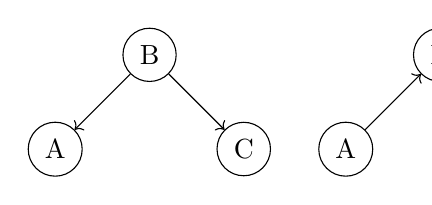
\begin{tikzpicture}[
			node distance=1cm,
			every node/.style={draw, circle}
			]
			% Graph A -> B -> C
			\node (B1) {B};
			\node (A1) [below left=of B1] {A};
			\node (C1) [below right=of B1] {C};
			
			\draw[->] (B1) -- (A1);
			\draw[->] (B1) -- (C1);
			
			\hspace{2cm}
			
			% Graph A <- B -> C
			\node (B2) [right=of B1] {B};
			\node (A2) [below left=of B2] {A};
			\node (C2) [below right=of B2] {C};
			
			\draw[->] (A2) -- (B2);
			\draw[->] (B2) -- (C2);
		\end{tikzpicture}
	\end{center}
	
	For both graphs above:
	\begin{itemize}
		\item A is independent of C conditioned on B
		\item C is independent of A conditioned on B
		\item None of the other variables is independent of B
	\end{itemize}
	
	If graphs $\mathcal{G}_0, \mathcal{G}_1$ contain the same independencies, they are in the same Markov equivalence class. \\
	
	A probability distribution $P$ is said to be \textbf{faithful} to a directed acyclic graph $\mathcal{G}$ if every conditional independence that holds in $P$ is implied by the d-separation criterion in $\mathcal{G}$. That is, for all disjoint sets $X, Y, Z \subseteq V$,
	$$X \indep Y \mid Z \text{ in } P \implies X \text{ and } Y \text{ are d-separated by } Z \text{ in } \mathcal{G}.$$
	Faithfulness ensures that the graph structure captures all and only the conditional independencies present in the distribution. \\
	
	Finally, we restate \textbf{Causal Sufficiency}: all confounders of the relevant variables are observed in the given dataset. \\
	
	Corollary: edges in the DAG imply causal relationships.
	
	\subsection{Causal Assumptions}
	
	Causal assumptions are necessary to ensure that the conclusions drawn from data analysis are valid and meaningful. They help to clarify the relationships between variables, address potential biases, and provide a framework for causal inference. Without these assumptions, we risk making erroneous conclusions based on observational data alone. Common assumptions are:
	
	\begin{enumerate}
		\item Faithfulness
		\item Acyclic data generating mechanisms (no feedback loops).
		\item No conditioning on unobserved colliders.
		\item No unobserved confounding (can be relaxed as in FCI \cite{fci2001}).
	\end{enumerate}
	
	Key Idea: Estimate the CPDAG from data, as causal relationships produce conditional independencies that can be utilized to reconstruct aspects of the causal model, specifically its Markov equivalence class.
	
	\subsection{Causal Structure Learning Algorithms}
	
	Causal structure learning algorithms are crucial for uncovering the causal relationships among variables from observational data. The PC algorithm (Peter \& Clark) is a prominent method that identifies these relationships by detecting conditional independencies, constructing a DAG to represent the causal structure \cite{pc1991}. Additionally, the Greedy Equivalence Search (GES) algorithm \cite{ges2024} optimizes the search for the best scoring DAG, while the Fast Causal Inference (FCI) algorithm \cite{fci2001} extends the capabilities of the PC algorithm to account for latent variables and unobserved confounding. Here, we will only recall the PC algorithm from \cite{pc1991}:
	
	\subsubsection*{PC Algorithm}
	
	For $a, b \in V$, let $A_{a,b}^\mathcal{G} = \{u \mid u \notin \{a, b\} \land (u \leftrightarrow a \in E \lor u \leftrightarrow b \in E)\}$ and $U_{a,b}^\mathcal{G} = \{u \mid u \notin \{a, b\} \land \exists aup_{a,b} \in G\}$. $A_{a,b}^\mathcal{G}$ and $U_{a,b}^\mathcal{G}$ are constantly changing as the algorithm progresses, as $\mathcal{G} = (V, E)$ is continually updated.
	\begin{algorithm}
		\caption{PC Algorithm}
		\begin{algorithmic}[1]
			\State \textbf{Input:} Set of vertices $ V $
			\State \textbf{Output:} all graphs (which are actually CPDAGs) with these orientations
			\State \textbf{Part A:}
			\State Form the complete undirected graph $ \mathcal{G} $ on $ V $: 
			\State \quad $ E := \{\{u_i, u_j\} \mid u_i, u_j \in V \} $
			
			\State \textbf{Part B:}
			\State $n := 0$
			\Repeat
				\ForAll {$(a, b) \in E$}
					\If {$|A_{a,b}^{\mathcal{G}} \cap U_{a,b}^{\mathcal{G}}| \geq n$ \textbf{and} $a \indep b \mid \{S \mid S \subseteq A_{a,b}^{\mathcal{G}} \cap U_{a,b}^{\mathcal{G}} \land |S| = n\}$}
						\State delete $(a, b)$ from $E$
					\EndIf
				\EndFor
				\State $n := n + 1$
			\Until{$\forall (a,b) \in E,\, |A_{a,b}^{\mathcal{G}} \cap U_{a,b}^{\mathcal{G}}| < n$}
			\State Call the resulting undirected graph $ F $
			
			\State \textbf{Part C:}
			\ForAll {$\{a, b, c \in V \mid (a,b), (b,c) \in F \land (a,c) \notin F\}$}
				\If{$\forall S \subseteq A_{a,b}^{\mathcal{G}} \cap U_{a,b}^{\mathcal{G}},\, b \in S: a \nindep c \mid S $}
					\State Orient $a \leftrightarrow b \leftrightarrow c$ as $a \rightarrow b \leftarrow c$
				\EndIf
			\EndFor
		\end{algorithmic}
	\end{algorithm}
	
	Additionally, one would implement Meek's orientation rules \cite{meek1995} for correctness and completeness: no incorrect orientations occur, and no further orientations can be made (See \autoref{fig:meeks_orientation}).
	
	Intuitively, one could interpret Part B of the PC algorithm as eliminating as many edges as possible using conditional independence tests. In Part C, the algorithm establishes causal directions for each remaining edge by considering colliders, the assumption that there are no cycles, and any additional arbitrary assumptions.
	
	\begin{figure}[H]
		\centering
		\includegraphics[width=0.75\textwidth]{Meek's Orientation Rules} 
		\caption{Meek's Orientation Rules from \cite{petersen2024}}
		\label{fig:meeks_orientation}
	\end{figure}
	
	Using PC on empirical data requires either a significance level to use in the tests or a conditional independence test. For the former, we do not have a principled approach for choosing the appropriate significance level; for the latter, there does not exist a generally correct test of conditional independence that does not rely on some distributional assumptions \cite{shah2020}.
		
	If the data is entirely categorical, we can directly test \textbf{conditional independence} by use of. a $\chi^2$ test of independence on the multi-way cross tabulation over $X, Y, Z$.
	
	For mix of binary and numerical variables, one might test
	for non-association using GLMs with spline-expansions \cite{petersen2021}.
	
	For the special case when the data are jointly normally distributed, we have $X \indep Y \mid Z \Leftrightarrow \text{cor}(X, Y \mid Z) = 0$ which is equivalent with testing null hypothesis $H_0 : \beta = 0$ in the linear regression model $Y_i = \alpha + \beta \cdot \X_i + \gamma \cdot Z_i + \epsilon_i$. \\
	
	The \textbf{significance level} used for individual tests in the PC algorithm is not a proper significance level for the globally estimated graph, as it does not describe the overall risk of a Type I error. Furthermore, if many tests are conducted and the result of one test informs which test should be conducted next, this implies a complicated multiple testing issue without obvious solutions. As with everything in statistics, we typically default to a significance level of $\alpha = 0.05$.
	 
	\subsection{Formal Definition of SCM}
	
	Causal graphs are DAGs that depict causal relationships in a binary manner. There is either a cause-effect relationship between two variables (indicated by an edge between them) or there is not. It would be more informative to have a model that includes more details about the causal relationship, such as the ability to quantify the effect. Therefore, we need to formulate a set of equations that describe all causal relationships in our model. 
	
	Random noise represents the variability in data that cannot be explained by the model, arising from measurement errors, environmental factors, or inherent randomness. Including random noise (with a specific distribution) in our model can enhance its applicability to real-world scenarios.
	
	In \cite{peters2017}, SCMs are defined in following way: \\
	
	A \textbf{structural causal model (SCM)} $\C := (\mathbf{S}, P_\mathbf{N})$ consists of:
	\begin{enumerate}
		\item a collection $\mathbf{S}$ of $d$ structural assignments
		$$
		\X_j := f_j(\mathbf{PA}_j, N_j), \quad j \in \{1, \dots, d\},
		$$
		where each $\mathbf{PA}_j \subseteq \{\X_1, \dots, \X_d\} \setminus \{\X_j\}$ is the set of parents of $\X_j$;
		\item a joint distribution $P_\mathbf{N} = P_{N_1, \dots, N_d}$ over the noise variables, which are assumed to be mutually independent, i.e.,
		$$
		P_\mathbf{N} = \prod_{j=1}^d P_{N_j}.
		$$
	\end{enumerate}
	
	Notice the assignment operator $:=$ in the definition. This is similar to assignment in programming, where we can change the value of a (random) variable at any time. This will be useful for interventions.
	
	Structural Causal Models (SCMs) are inherently probabilistic due to the presence of random noise terms, which we assume to be independent. We posit that our model adequately captures all systematic dependencies within the system, leaving no unobserved confounding factors. Should unobserved confounding exist, it would necessitate the inclusion of additional unobserved nodes or a generalization of the SCM framework.
	
	\subsubsection*{Structural Minimality}
	
	Definition of SCMs currently distinguishes between: $$S_1: X := N_x, Y = 0 \cdot X + N_y, \quad S_2: X := N_x, Y := N_Y$$ As this contradicts our intuition, we add the requirement that the functions $f_j$ depend on all of their input arguments: For $k \in \{1, \dots, d\}$, a function $g$ and a minimal (with respect to set size) subset $\mathbf{PA}_k^-$ such that: $$f_k (\mathbf{PA}_k, N_k) = g(\mathbf{PA}_k^-, N_k), \quad \forall \mathbf{PA}_k, N_k \text{ with } P(N_k) > 0 \text{ and } \mathbf{PA}_k^- \subsetneq \mathbf{PA}_k$$
	
	In this case, we always choose the latter representation; thus, with this definition of structural minimality, one would choose $S_2$ over $S_1$. We assume that structural minimality always holds.
	
	\subsection{From Causal Graph to SCM}

	If a causal graph is constructed by following the aforementioned steps, the quantification step can be achieved through various methodologies from classical statistics and machine learning. Each function $f_i$ may be learned using techniques such as artificial neural networks (ANNs), ordinary least squares, decision trees, or neural networks, which are recognized as the state-of-the-art methods for general structural causal model estimation.
	
	Nevertheless, it is necessary to evaluate the assumptions that can be made (for instance, linearity in the case of ordinary least squares), substantiate these assumptions with theoretical foundations, and implement suitable models accordingly.
	
	\subsection{Interventions}
	
	Interventional questions are central to causal inference, inquiring about the effects of setting one or more variables to specific values. These questions describe interventions, which involve altering a system by forcing variables to adopt designated values.
	
	This process of intervening is fundamentally different from conditioning, which involves selecting observations based on certain values while ignoring others. Intervening requires all instances to adopt a specified value. As a result, the expression $P(Y \mid \boldsymbol{do}(\X_j := k))$, representing the probability distribution of $Y$ when $\X_j$ is set to a specific value, does not generally equal the conditional probability $P(Y \mid \X_j = k)$.
	
	Because conditioning and intervening are not equivalent, interventional questions cannot be addressed simply by comparing means. SCMs are particularly valuable in this context, as they facilitate the modeling of intervention distributions when proper causal discovery has been conducted or when expert knowledge of the qualitative graph is available. After intervening on a variable, we assert that the new SCM entails a new distribution known as the interventional distribution. \\
	
	\textbf{Formal Definition:}
	
	Given a SCM $\C$ with endogenous variables $\X_1, \dots, \X_n$, an intervention $\C^{\boldsymbol{do}(\X_i := k)}$ denotes an external manipulation that sets $\X_i$ to the value $k$, irrespective of its natural causes. \\
	
	\textbf{Mechanics:}
	
	Applying the intervention $\boldsymbol{do}(\X_i := k)$ to the SCM corresponds to:
	\begin{itemize}
		\item Replacing the structural equation for $\X_i$ with a constant assignment: $\X_i := k$.
		\item Removing all incoming edges into $\X_i$ in the associated causal graph.
	\end{itemize}
	
	To address challenges such as the uncertainty regarding the identification of causal variables, please refer to \cite{subramanian2022}.
	
	\section{Diffusion Probabilistic Models}
	
	From \cite{chan2025}: "The astonishing growth of generative tools in recent years has empowered many exciting applications in text-to-image and text-to-video generation. The underlying principle behind these generative tools is the concept of \textit{diffusion}, a particular sampling mechanism that has overcome some longstanding shortcomings in previous approaches".
	
	Sohl-Dickstein et al. \cite{sohl-dickstein2015} proposed constructing a chain of conversions instead of a one-step
	process of variational auto-encoder (VAE) \cite{kingma2014}. 	We define $\x_{0:T} = \{\x_0, \dots, \x_T\}$ as collection of all state variables from $t = 0$ to $t = T$. Analogous to the encoder and decoder architecture of VAE, they defined forward and reverse processes. In both cases, they consider a sequence of variables $\x_0, \dots, \x_T$ whose joint distribution is denoted as $q_\phi (\x_{0:T})$ and $p_\theta (\x_{0:T})$ respectively for the forward and reverse processes. Again, analogous to the VAE, the true transition distribution $p(\x_t \mid \x_{t+1})$ (as well as $p(\x_t \mid \x_{t-1})$) is not accessible, so we approximate it with $q_\phi(\x_{0:T})$ and $p_\theta(\x_{0:T})$. To ensure computational tractability, the Markov property is imposed on both processes: 
	
	$$\text{Forward(} \x_0 \to \x_T \text{): } q_\phi (\x_{0:T}) = q(\x_0) \prod_{t=1}^{T} q_\phi (\x_t \mid \x_{t-1})$$
	$$\text{Reverse(} \x_T \to \x_0 \text{): } p_\theta (\x_{0:T}) = p(\x_T) \prod_{t=1}^{T} p_\theta (\x_{t-1} \mid \x_t)$$
	
	Since transition distributions depend only on their immediate previous state, the overall generation process is broken down into many smaller tasks. The same neural network will be used for $T$ times. This "Divide and Conquer" strategy allows us to use simpler distributions at each step. The properties of a Gaussian ensure that the posterior will remain a Gaussian if both the likelihood and the prior are Gaussian. Since a Gaussian depends only on two hyperparameters, namely mean and variance, it is highly tractable. \\
	
	\begin{figure}[htb]
		\centering
		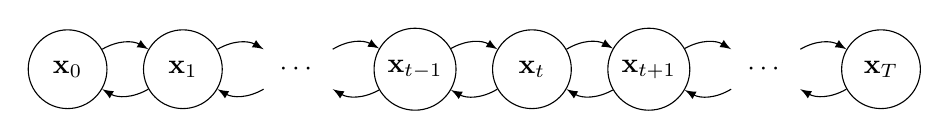
\begin{tikzpicture}[>=latex, node distance=0.45cm, every node/.style={circle,draw,minimum size=1cm}]
			% Nodes
			\node (x0)           {$\x_0$};
			\node (x1) [right=of x0] {$\x_1$};
			\node (dotsl) [right=of x1, draw=none] {$\cdots$};
			\node (xtm) [right=of dotsl] {$\x_{t-1}$};
			\node (xt)  [right=of xtm]  {$\x_t$};
			\node (xtp) [right=of xt]   {$\x_{t+1}$};
			\node (dotsr) [right=of xtp, draw=none] {$\cdots$};
			\node (xT) [right=of dotsr] {$\x_T$};
			% Edges: upper (forward)
			\foreach \src/\dst in {x0/x1,x1/dotsl,dotsl/xtm,xtm/xt,xt/xtp,xtp/dotsr,dotsr/xT}
			{\draw[->] (\src) to[bend left=30] (\dst);}
			% Edges: lower (backward)
			\foreach \src/\dst in {x1/x0,dotsl/x1,xtm/dotsl,xt/xtm,xtp/xt,dotsr/xtp,xT/dotsr}
			{\draw[->] (\src) to[bend left=30] (\dst);}
		\end{tikzpicture}
		\caption{Variational Diffusion Model}
		\label{fig:variational-diffusion-model}
	\end{figure}
	
	\subsection{Variational Auto Encoder}
	
	VAE-inspired diffusion model is, unsurprisingly, called the \textbf{variational diffusion model} (see \autoref{fig:variational-diffusion-model}). In this model, $\x_0$ corresponds to the input $\x$ in the VAE, $\x_T$ corresponds to the latent variable $z$, and $\x_i$, for all $i \in \{1, \dots, T - 1\}$, are (latent) intermediate states.
	
	In a variational diffusion model (and also DDPM which we will discuss later), the (Gaussian) transition distribution is defined as: $$q (\x_t \mid \x_{t-1}) := \mathcal{N}(\x_t \mid \sqrt{\alpha_t} \x_{t-1}, (1 - \alpha_t) \mathbb{I})$$
	
	The mean is $\sqrt{\alpha_t} \x_{t-1}$ and the variance is $(1 - \alpha_t)$. The choice of the scaling factor $\sqrt{\alpha_t}$ is to make sure that the variance magnitude is preserved so that it will not explode and vanish after many iterations.
	
	Conditional distribution $q_\phi (\x_t \mid \x_0)$ is given by: $$q_\phi (\x_t \mid \x_0) = \mathcal{N}(\x_t \mid \sqrt{\bar{\alpha}_t} \x_0, (1 - \sqrt{\bar{\alpha}_t}) \mathbb{I}) \text{ with } \bar{\alpha}_t = \prod_{i=1}^t \alpha_i$$
	
	A common point of confusion is why we need to derive transition distributions such as $q_\phi(\x_t \mid \x_{t-1})$ and $q_\phi(\x_t \mid \x_0)$ if the apparent goal is simply to map an input $p(\x_0)$ to white noise $p(\x_T)$. This is because these distributions define the forward diffusion process, where the data is iteratively corrupted by Gaussian noise in a Markov chain, leading eventually to an standard normal distribution as $T$ becomes large. Importantly, the forward process is constructed to be analytically tractable, allowing us to express transitions like $q_\phi(\x_t \mid \x_0)$ in closed form. The reverse process, which is the focus of training and generation, relies on these closed-form expressions and Markov structure to define and couple each denoising step to its corresponding forward step. Thus, $q_\phi(\x_t \mid \x_0)$ provides a convenient and formally grounded way to describe and implement the forward process, serving as the foundation for learning to reverse the transformation from noise back to meaningful data.
	
	\subsubsection*{ELBO}
	
	Recall the loss function for VAE, evidence lower bound (ELBO) from \cite{kingma2014}. For variational diffusion model, ELBO is defined as (with $\x_0 = \x$, $\x_1 \sim q_\phi(\x_1 \mid \x_0)
	$ and $\x_T \sim \N(0, \mathbb{I}))$:
	
	$$\begin{aligned}
		\mathcal{L}_{\phi, \theta} (\x) =\ & 
		\E_{q_\phi(\x_1 \mid \x_0)} 
		\left[ \log p_\theta(\x_0 \mid \x_1) \right] \\
		& - \mathbb{E}_{q_\phi(\x_{T-1} \mid \x_0)} 
		\left[ \D_{\mathrm{KL}} \left( q_\phi(\x_T \mid \x_{T-1}) \dklbar p(\x_T) \right) \right] \\
		& - \sum_{t=1}^{T-1} \E_{q_\phi(\x_{t-1}, \x_{t+1} \mid \x_0)} 
		\left[ \D_{\mathrm{KL}} \left( q_\phi(\x_t \mid \x_{t-1}) \dklbar p_\theta(\x_t \mid \x_{t+1}) \right) \right]
	\end{aligned}$$
	
	The first expected value measures how good the initial block is, the second expected value measures how good the final block is, and the sum of the remaining expected values measures how good the intermediate blocks are. \\
	
	\textbf{Why expectation?} $p_\theta(\x_0 \mid \x_1)$ is a function of $\x_1$, so for different values of $\x_1$, the value of $p_\theta(\x_0 \mid \x_1)$ will differ. Taking the expectation removes the dependency on $\x_1$.
	
	In prior matching, the KL divergence measures the difference between $q_\phi(\x_T \mid \x_{t-1})$ and $p(\x_T)$. We use the conditional distribution $q_\phi(\x_{T-1} \mid \x_0)$ because $\x_{T-1}$ depends on $\x_0$. The expectation over $q_\phi(\x_{T-1} \mid \x_0)$ provides the KL divergence value for each $\x_{T-1}$ sampled from $q_\phi(\x_{T-1} \mid \x_0)$ and also eliminates the dependency. The same reasoning applies to the intermediate transition blocks.\\
	
	The challenge with the intermediate transition block of the loss function is that we need to sample $(\x_{t-1}, \x_{t+1})$ from the joint distribution $q_\phi(\x_{t-1}, \x_{t+1} \mid \x_0)$, which is unknown. Even though it is Gaussian by design, we cannot sample future values of $\x_{t+1}$. 
	
	By conditioning on $\x_0$, and applying Bayes' theorem, we get:
	$$
	q_\phi(\x_t \mid \x_{t-1}, \x_0) = \frac{q_\phi(\x_{t-1} \mid \x_t, \x_0)\, q_\phi(\x_t \mid \x_0)}{q_\phi(\x_{t-1} \mid \x_0)}.
	$$
	
	Without conditioning on $\x_0$, we cannot sample from $q(\x_{t-1})$, since $\x_{t-1}$ depends on the initial input $\x_0$. Now, we can switch from $q_\phi(\x_t \mid \x_{t-1}, \x_0)$ to $q_\phi(\x_{t-1} \mid \x_t, \x_0)$. This avoids handling two opposing directions and still allows us to check for consistency across transition blocks. The direction $q_\phi(\x_{t-1} \mid \x_t, \x_0)$ aligns with $p_\theta(\x_{t-1} \mid \x_t)$.
	$$\begin{aligned}
		\mathcal{L}_{\phi, \theta} (\x) =\ & 
		\E_{q_\phi(\x_1 \mid \x_0)} 
		\left[ \log p_\theta(\x_0 \mid \x_1) \right] \\
		& - \D_{\mathrm{KL}} \left( q_\phi(\x_T \mid \x_{0}) \dklbar p(\x_T) \right) \\
		& - \sum_{t=2}^{T} \E_{q_\phi(\x_{t} \mid \x_0)} 
		\left[ \D_{\mathrm{KL}} \left( q_\phi(\x_{t-1} \mid \x_t, \x_0) \dklbar p_\theta(\x_{t-1} \mid \x_t) \right) \right]
	\end{aligned}$$
	
	The initial block remains unchanged. Prior matching has been simplified to the KL divergence between $q_\phi(\x_T \mid \x_0)$ and $p(\x_T)$, since we now condition on $\x_0$ and there is no need to sample from $q_\phi(\x_{T-1} \mid \x_0)$ or take an expectation over it.
	
	The new consistency term differs from the previous one in two key ways. First, the running index $t$ starts at $t = 2$ and ends at $t = T$. Second, the distribution matching is now performed between $q_\phi(\x_{t-1} \mid \x_0)$ and $p_\theta(\x_{t-1} \mid \x_t)$. Thus, instead of requiring the forward transition to match the reverse transition, we use $q_\phi$ to construct a reverse transition and match it with $p_\theta$. \\
	
	\textbf{Distribution of $q_\phi (\x_{t-1} \mid \x_t, \x_0)$} takes the form of $q_\phi (\x_{t-1} \mid \x_t, \x_0) = \N(\x_{t-1} \mid \boldsymbol{\mu}_q (\x_t, \x_0), \boldsymbol{\Sigma}_q (t))$ where: $$\boldsymbol{\mu}_q (\x_t, \x_0) = \frac{(1 - \bar{\alpha}_{t-1}) \sqrt{\alpha_t}}{1 - \bar{\alpha}_t} \x_t + \frac{(1 - \alpha_t) \sqrt{\bar{\alpha}_{t-1}}}{1 - \bar{\alpha}_t} \x_0$$
	$$\boldsymbol{\Sigma}_q (t) = \frac{(1 - \alpha_t) (1 - \sqrt{\bar{\alpha}_{t-1}})}{1 - \bar{\alpha}_t} \mathbb{I} =: \sigma_q^2 (t) \mathbb{I}$$
	where $\bar{\alpha}_t = \prod_{i=1}^t \alpha_i$. For the proof, see page 30 of \cite{chan2025}. \\
	
	Note that $q_\phi(\x_{t-1} \mid \x_t, \x_0)$ is fully determined by $\x_t$ and $\x_0$, and is not learned through a neural network, unlike in a VAE. There is no statistical learning involved if the hyperparameter $\alpha_t$ is provided.
	
	We now turn our attention to $p_\theta(\x_{t-1} \mid \x_t)$. Since $q_\phi(\x_{t-1} \mid \x_t, \x_0)$ is Gaussian, we choose $p_\theta(\x_{t-1} \mid \x_t)$ to also be Gaussian, allowing for efficient computation of the KL divergence. Specifically, we define
	\[
	p_\theta(\x_{t-1} \mid \x_t) = \N(\x_{t-1} \mid \boldsymbol{\mu}_\theta(\x_t), \sigma_q^2(t)\, \mathbb{I}),
	\]
	where $\boldsymbol{\mu}_\theta(\x_t)$ is a neural network.
	
	The KL divergence is simplified to:
	\begin{align*}
		&\D_{\mathrm{KL}}\left( q_\phi(\x_{t-1} \mid \x_t, \x_0) \dklbar p_\theta(\x_{t-1} \mid \x_t) \right) \\
		& \qquad = \D_{\mathrm{KL}}\left(
		\N\left(\x_{t-1} \mid \boldsymbol{\mu}_q(\x_t, \x_0), \sigma_q^2(t)\, \mathbb{I}\right)
		\dklbar
		\N\left(\x_{t-1} \mid \boldsymbol{\mu}(\x_t), \sigma_q^2(t)\, \mathbb{I}\right)
		\right) \\
		& \qquad = \frac{1}{2 \sigma_q^2(t)} \left\lVert 
		\boldsymbol{\mu}_q(\x_t, \x_0) - \boldsymbol{\mu}(\x_t)
		\right\rVert^2
	\end{align*}
	
	For the ELBO, the dependency on $\phi$ is dropped because $q_\phi$ depends only on $\x_t$ and $\x_0$, which are not learned:
	$$\begin{aligned}
		\mathcal{L}_{\theta} (\x) =\ & 
		\E_{q (\x_1 \mid \x_0)} 
		\left[ \log p_\theta(\x_0 \mid \x_1) \right] \\
		& - \D_{\mathrm{KL}} \left( q (\x_T \mid \x_{0}) \dklbar p(\x_T) \right) \\
		& - \sum_{t=2}^{T} \E_{q (\x_{t} \mid \x_0)} 
		\left[ \lVert 
		\boldsymbol{\mu}_q(\x_t, \x_0) - \boldsymbol{\mu}(\x_t)
		\rVert^2 \right]
	\end{aligned}$$
	
	with $\x = \x_0$ and $\x_T \sim \N (0, \mathbb{I})$. \\
	
	The reconstruction term (initial block) can be further simplified:
	\begin{align*}
		\log p_\theta (\x_0 \mid \x_1) & = \log \N(\x_0 \mid \boldsymbol{\mu}_\theta (\x_1), \sigma_q^2 (1) \mathbb{I}) \\ & = \log \frac{1}{\sqrt[d]{2 \pi \sigma_q^2 (1)}} \exp \left\{ - \frac{\lVert \x_0 - \boldsymbol{\mu}_\theta (\x_1) \rVert^2}{2 \sigma_q^2 (1)} \right\} \\ & = - \frac{\lVert \x_0 - \boldsymbol{\mu}_\theta (\x_1) \rVert^2}{2 \sigma_q^2 (1)} - \frac{d}{2} \log (2 \pi \sigma_q^2 (1))
	\end{align*}

	\subsection{Denoising Diffusion Probabilistic Model}

	Recall $\displaystyle \boldsymbol{\mu}_q (\x_t, \x_0) = \frac{(1 - \bar{\alpha}_{t-1}) \sqrt{\alpha_t}}{1 - \bar{\alpha}_t} \x_t + \frac{(1 - \alpha_t) \sqrt{\bar{\alpha}_{t-1}}}{1 - \bar{\alpha}_t} \x_0$. Defining $\displaystyle \boldsymbol{\mu}_\theta (\x_t) := \frac{(1 - \bar{\alpha}_{t-1}) \sqrt{\alpha_t}}{1 - \bar{\alpha}_t} \x_t + \frac{(1 - \alpha_t) \sqrt{\bar{\alpha}_{t-1}}}{1 - \bar{\alpha}_t} \hat{\x}_\theta (\x_t)$, where $\hat{\x}_\theta (\x_t)$ is another network, we can rewrite $$\displaystyle \frac{1}{2 \sigma_q^2(t)} \lVert 
	\boldsymbol{\mu}_q(\x_t, \x_0) - \boldsymbol{\mu}(\x_t)
	\rVert^2$$ as $$\displaystyle \frac{1}{2 \sigma_q^2(t)} \frac{(1 - \alpha_t)^2 \bar{\alpha}_{t-1}}{(1 - \bar{\alpha}_t)^2} \lVert \hat{\x}_\theta (\x_t) - \x_0 \rVert^2$$
	
	Using the above, and incorporating $\E_{q (\x_1 \mid \x_0)} \left[\log p_\theta (\x_0 \mid \x_1) \right]$ into the summation, we obtain the ELBO for denoising diffusion probabilistic model (with $\bar{\alpha}_t = \prod_{i=1}^t \alpha_i$) as: $$\mathcal{L}_\theta^{\mathrm{DDPM}} = - \sum_{t=1}^{T} \frac{1}{2 \sigma_q^2(t)} \frac{(1 - \alpha_t)^2 \bar{\alpha}_{t-1}}{(1 - \bar{\alpha}_t)^2} \E_{q (\x_t \mid \x_0)} \left[ \lVert \hat{\x}_\theta (\x_t) - \x_0 \rVert^2 \right]$$
	
	For the proof, see page 34 of \cite{chan2025}. \\
	
	Using Monte Carlo approximation of expectation, we can rewrite the optimization problem: $\arg\max_\theta \sum_{\x_0 \in \mathcal{X}} \mathcal{L}_\theta^{\mathrm{DDPM}}$ as
	$$ \arg\min_\theta \sum_{\x_0 \in \mathcal{X}} \sum_{t=1}^T \frac{1}{M} \frac{1}{2 \sigma_q^2(t)} \frac{(1 - \alpha_t)^2 \bar{\alpha}_{t-1}}{(1 - \bar{\alpha}_t)^2} \left\lVert \hat{\x}_\theta \left(\sqrt{\bar{\alpha}_t} \x_0 + \sqrt{1 - \bar{\alpha}_t} \, \boldsymbol{\epsilon}_t^{(m)} \right) - \x_0 \right\rVert^2 $$
	where $\boldsymbol{\epsilon}_t^{(m)} \sim \N (0, \mathbb{I})$ and $\mathcal{X}$ is the training set. This loss function has $\hat{\x}_0 (\cdot)$ which is a denoiser, so this model is called the denoising diffusion probabilistic model (DDPM).
	
	\subsubsection*{Training DDPM}
	
	The forward diffusion in DDPM generates intermediate variables $\x_{1:T-1}$ by sampling $$ \x_t \sim q(\x_t \mid \x_0) = \N \left( \x_t \mid \sqrt{\bar{\alpha}_t} \x_0,\ (1 - \bar{\alpha}_t) \mathbb{I} \right) \Rightarrow \x_t = \sqrt{\bar{\alpha}_t} \x_0 + \sqrt{1 - \bar{\alpha}_t} \, \boldsymbol{\epsilon}, \boldsymbol{\epsilon} \sim \N (0,\, \mathbb{I}).$$
	The forward diffusion process requires no training. Given an input $\x_0$, it produces the entire sequence $\x_{1:T}$. We train a single denoiser network to handle all noise levels, since each $\x_t$ corresponds to a noise level with a different variance $1 - \bar{\alpha}_t$. Training separate denoisers for each time step is computationally infeasible due to the high dimensionality of $T$
	
	\begin{algorithm}
	\caption{Training Algorithm for DDPM}
	\begin{algorithmic}[1]
		\Repeat
			\State $\x_0 \sim q(\x_0)$ ($\x_0 \in \mathcal{X}$)
			\State $t \sim \text{ Uniform}[1, T]$ (time stamp)
			\State $\boldsymbol{\epsilon}_t^{(m)} \sim \N (0, \mathbb{I})$
			\State $\x_t^{(m)} = \bar{\alpha}_t \x_0 + \sqrt{1 - \bar{\alpha}_t} \boldsymbol{\epsilon}_t^{(m)}$
			\State Take gradient step on $\nabla_\theta \left\{ \frac{1}{M} \sum_{m=1}^M \lVert \hat{\x}_\theta (\x_t^{(m)}) - \x_0 \rVert^2 \right\}$
		\Until{convergence}
	\end{algorithmic}
	\end{algorithm}
	
	\subsubsection*{Inference of DDPM}
	
	Once the denoiser $\hat{\x}_\theta$ is trained, we can do the inference. We sample from $p_\theta (\x_{t-1} \mid \x_t)$ over the sequence of states $\x_T, \x_{T-1}, \dots, \x_1$. $$\x_{t-1} \sim p_\theta (\x_{t-1} \mid \x_t) = \N (\x_{t-1} \mid \boldsymbol{\mu}_\theta (\x_t), \sigma_q^2 (t) \mathbb{I})$$
	By reparameterization, we have (for $\boldsymbol{\epsilon} \sim \N(0, \mathbb{I})$): $$\x_{t-1} = \boldsymbol{\mu}_\theta (\x_t) + \sigma_q (t) \boldsymbol{\epsilon} = \frac{(1 - \bar{\alpha}_{t-1}) \sqrt{\alpha_t}}{1 - \bar{\alpha}_t} \x_t + \frac{(1 - \alpha_t) \sqrt{\bar{\alpha}_{t-1}}}{1 - \bar{\alpha}_t} \hat{\x}_\theta (\x_t) + \sigma_q (t) \boldsymbol{\epsilon}$$
	
	Using the reparameterization above, we run the denoiser $T$ times, starting from the white noise vector $\x_T$ and iteratively denoising back to an estimate of the original input $\bar{\x}_0$.
	
	\begin{algorithm}
		\caption{Inference Algorithm for DDPM}
		\begin{algorithmic}[1]
			\State \textbf{Given:} $\x_T \sim \N (0, \mathbb{I})$
			\For{$t = T, T - 1, \dots, 1$}
				\State $\boldsymbol{\epsilon}_t^{(m)} \sim \N (0, \mathbb{I})$
				\State $\displaystyle \x_{t-1} = \frac{(1 - \bar{\alpha}_{t-1}) \sqrt{\alpha_t}}{1 - \bar{\alpha}_t} \x_t + \frac{(1 - \alpha_t) \sqrt{\bar{\alpha}_{t-1}}}{1 - \bar{\alpha}_t} \hat{\x}_\theta (\x_t) + \sigma_q (t) \boldsymbol{\epsilon}$
			\EndFor
		\end{algorithmic}
	\end{algorithm}
	
	\subsection*{Useful insights from \cite{ho2020}}
	
	We will skip the derivation (algebraic) steps, which can be found in~\cite{ho2020}, but we highlight a few useful insights below:
	
	\subsubsection*{We can learn to predict noise}
	$$\x_t = \sqrt{\bar{\alpha}_t} \x_0 + \sqrt{1 - \bar{\alpha}_t} \boldsymbol{\epsilon}_0 \implies \x_0 = \frac{\x_t - \sqrt{1 - \bar{\alpha}_t} \boldsymbol{\epsilon}_0 }{\sqrt{\bar{\alpha}_t}}$$
	From this, we obtain the following equivalent expressions:
	$$\boldsymbol{\mu}_q (\x_t, \x_0) = \frac{1}{\sqrt{\alpha}_t} \x_t - \frac{1 - \alpha_t}{\sqrt{1 - \bar{\alpha_t}} \sqrt{\alpha_t}} \boldsymbol{\epsilon}_0$$
	$$\boldsymbol{\mu}_\theta (\x_t) = \frac{1}{\sqrt{\alpha}_t} \x_t - \frac{1 - \alpha_t}{\sqrt{1 - \bar{\alpha_t}} \sqrt{\alpha_t}} \boldsymbol{\hat{\epsilon}}_0 (\x_t)$$
	This is useful, as we have expressed $\boldsymbol{\mu}_q(\x_t, \x_0)$ as a function of $\boldsymbol{\epsilon}_0$ rather than $\x_0$. Substituting this into the new ELBO:
	$$\mathcal{L}_\theta^{\mathrm{DDPM}} (\x_0, \boldsymbol{\epsilon}_0) = - \sum_{t=1}^{T} \E_{q (\x_t \mid \x_0)} \left[ \frac{1}{2 \sigma_q^2(t)} \frac{(1 - \alpha_t)^2 }{(1 - \bar{\alpha}_t)^2 \alpha_t} \lVert \boldsymbol{\hat{\epsilon}}_0 \left( \sqrt{\bar{\alpha}_t} \x_0 + \sqrt{1 - \bar{\alpha}_t} \boldsymbol{\epsilon}_0 \right) - \boldsymbol{\epsilon}_0 \rVert^2 \right] $$
	As this ELBO is a function of $\x_0$ and $\boldsymbol{\epsilon}_0$, we need to solve the following optimization problem: $$\arg\min_\theta \sum_{\x_0 \in \mathcal{X}} \frac{1}{M} \sum_{m=1}^{M} \mathcal{L}_\theta^{\mathrm{DDPM}} (\x_0, \boldsymbol{\epsilon}_0^{(m)})$$
	
	\begin{algorithm}
		\caption{Training Algorithm for DDPM (using $\hat{\epsilon}_\theta (\x_t)$)}
		\begin{algorithmic}[1]
			\Repeat
			\State $\x_0 \sim q(\x_0)$ ($\x_0 \in \mathcal{X}$)
			\State $t \sim \text{ Uniform}[1, T]$ (time stamp)
			\State $\boldsymbol{\epsilon}_t^{(m)} \sim \N (0, \mathbb{I})$
			\State $\x_t^{(m)} = \bar{\alpha}_t \x_0 + \sqrt{1 - \bar{\alpha}_t} \boldsymbol{\epsilon}_t^{(m)}$
			\State Take gradient step on $\nabla_\theta \left\{ \lVert \hat{\epsilon}_\theta (\x_t) - \x_0 \rVert^2 \right\}$
			\Until{convergence}
		\end{algorithmic}
	\end{algorithm}
	
	\begin{algorithm}[H]
		\caption{Inference Algorithm for DDPM (using $\hat{\epsilon}_\theta (\x_t)$)}
		\begin{algorithmic}[1]
			\State \textbf{Given:} $\x_T \sim \N (0, \mathbb{I})$
			\For{$t = T, T - 1, \dots, 1$}
			\State $\boldsymbol{z} \sim \N (0, \mathbb{I})$
			\State $\displaystyle \x_{t-1} = \frac{1}{\sqrt{\alpha}_t} \left( \x_t - \frac{1 - \alpha_t}{\sqrt{1 - \bar{\alpha_t}}} \boldsymbol{\hat{\epsilon}}_0 (\x_t) \right) + \sigma_q (t) \boldsymbol{z}$
			\EndFor
		\end{algorithmic}
	\end{algorithm}
	
	\subsection*{Denoising Diffusion Implicit Model (DDIM)}
	
	A key drawback of DDPMs is their reliance on many iterations to generate high-fidelity samples. As noted by Song et al \cite{song2023}, a DDPM would take more than 1,000 hours to generate 50,000 $256 \times 256$ images on a standard GPU. This inefficiency arises because the reverse diffusion process requires iterative denoising; if the process intrinsically needs many steps to converge, generation will inherently be slow. Therefore, to accelerate computation, it is necessary to reduce the number of iterations. DDIM was introduced to address this limitation and provide faster image generation.
	
	\subsubsection*{Probability Distributions in DDIM}
	We introduced the Markov property for $q(\x_t \mid \x_{t-1})$ to make computation tractable; however, a key drawback is that a Markov chain often requires many steps to converge. DDIM addresses this issue by departing from the Markovian structure and adopting a non-Markovian formulation:
	$$q(\x_t \mid \x_{t-1}) := \N \left( \x_t \mid \sqrt{\frac{\alpha_t}{\alpha_{t-1}}} \x_{t-1}, \left( 1 - \frac{\alpha_t}{\alpha_{t-1}} \right) \mathbb{I} \right)$$
	Now, $\displaystyle \bar{\alpha}_t := \prod_{i=1}^t \frac{\alpha_i}{\alpha_{i-1}} = \alpha_t$ assuming $\alpha_0 = 1 $. 
	
	This implies: $q(\x_t \mid \x_0) = \N \left( \x_t \mid \sqrt{\alpha_t} \x_0, (1 - \alpha_t) \mathbb{I} \right)$. By means of reparameterization, we get $\x_t = \sqrt{\alpha_t} \x_0 + \sqrt{1 - \alpha_t} \boldsymbol{\epsilon}, \boldsymbol{\epsilon} \sim \N (0, \mathbb{I})$.
	
	The key idea is to rewrite the expression for $\eps$ so that $\x_{t-1}$ is no longer directly dependent on $\x_0$, which is perturbed by white noise. Starting from the standard forward diffusion equation:
	$$\x_t = \sqrt{\alpha_t} \x_0 + \sqrt{1 - \alpha_t} \, \eps$$
	we can rearrange it to isolate $\eps$:
	
	$$\eps = \frac{\x_t - \sqrt{\alpha_t}\, \x_0}{\sqrt{1 - \alpha_t}}$$
	
	Using the standard forward diffusion equation for $\x_{t-1}$ and substituting the expression for $\boldsymbol{\epsilon}$ derived above, we obtain: $$\x_{t-1} = \sqrt{\alpha_{t-1}} \x_0 + \sqrt{1 - \alpha_{t-1}} \frac{\x_t - \sqrt{\alpha_t}\, \x_0}{\sqrt{1 - \alpha_t}}$$
	
	While $\eps$ simplifies DDPMs, the Gaussian noise also slows the reverse diffusion process.
	
	Likely the most important argument in DDIM is that we desire the marginal distribution $q(\x_{t-1} \mid \x_0)$ to have the same form as $q(\x_t \mid \x_0)$. The motivation for aiming for this distribution is that, ultimately, we care about the marginal distribution $q(\x_t \mid \x_0)$, which we want to become pure white noise when $t = T$, and the original image when $t = 0$. Therefore, while we can have millions of different choices for the transition distribution $q(\x_{t-1} \mid \x_t, \x_0)$, only a few specialized transition probabilities can ensure that $q(\x_{t-1} \mid \x_0)$ takes a desirable form.
	
	Using equation 2.115 from \cite{bishop2006}, we get the \textbf{DDIM Transition Distribution}:
	$$q(\x_{t-1} \mid \x_t, \x_0) = \N \left( \sqrt{\alpha_{t-1}} \x_0 + \sqrt{1 - \alpha_{t-1} - \sigma_t^2} \left( \frac{\x_t - \sqrt{\alpha_t}\, \x_0}{\sqrt{1 - \alpha_t}} \right), \sigma_t^2 \mathbb{I} \right)$$
	If $q(\x_t \mid \x_0) = \N \left( \sqrt{\alpha_t} \x_0, (1 - \alpha_t) \mathbb{I} \right)$, then it follows from our derivation that $q(\x_{t-1} \mid \x_0) = \N \left( \sqrt{\alpha_{t-1}} \x_0, (1 - \alpha_{t-1}) \mathbb{I} \right)$.
	
	\subsubsection*{Inference for DDIM}

	The inference for DDIM is derived based on the transition distribution. Starting with the forward process, if we want to perform the reverse, we need to solve for $\x_0$ from the following equation: $$\x_t = \sqrt{\alpha_t} \, \x_0 + \sqrt{1 - \alpha_t} \, \eps$$
	where $\x_t$ is given, $\sqrt{1 - \alpha_t} \, \eps$ is estimated by the network, and our goal is to find $\sqrt{\alpha_t} \, \x_0$. By estimating the noise $\eps$ with $\eps_\theta^{(t)}(\x_t)$, which replaces $\eps$. We also define the estimate of the true signal $\x_0$ as:
	$$f_\theta^{(t)}(\x_t) := \frac{1}{\sqrt{\alpha_t}} \left( \x_t - \sqrt{1 - \alpha_t} \, \eps_\theta^{(t)}(\x_t) \right)$$
	
	We recall that this distribution is denoted by $q(\x_{t-1} \mid \x_t, \x_0)$. If we don't have access of $\x_0$, we replace it with $f_\theta^{(t)}(\x_t)$. Skipping derivations, we get for DDIM: $$\x_{t-1} = \sqrt{\alpha_{t-1}} \left( \frac{\x_t - \sqrt{1 - \alpha_t} \eps_\theta^{(t)} (\x_t)}{\sqrt{\alpha_t}} \right) + \sqrt{1 - \alpha_{t-1} - \sigma_t^2} \cdot \eps_\theta^{(t)} (\x_t) + \sigma_t \cdot \eps_t, \, \eps \sim \N (0, \mathbb{I})$$
	
	The main difference between DDPM and DDIM is subtle. While they both use $\x_t$ and $\eps^{(t)} (\x_t)$ in their
	updates, the specific update formula makes a different convergence speed. In fact, later in the differential
	equation literature where people connect DDIM and DDPM with stochastic differential equations, it was
	observed that DDIM employed some special accelerated first-order numerical schemes when solving the
	differential equation.
	
	\section{Score-Matching Langevin Dynamics \& Langevin and Fokker-Planck Equations}
	
	In this section, we briefly introduce the high-level intuition behind Score-Matching Langevin Dynamics as well as the Langevin and Fokker-Planck equations, which together form an important foundation for understanding the theory and practice of diffusion-based generative models. We will not go into detailed mathematical derivations or technical proofs for either topic; our focus is on building intuition for their roles and contributions. For readers interested in rigorous exposition and further technical details, we recommend \cite{vincent2011} and \cite{yang2019} for Score-Matching Langevin Dynamics (SMLD), and \cite{risken1989} for formal analysis of the Langevin and Fokker-Planck equations.
	
	\subsection{SMLD: Principles and Significance}
	
	Score-Matching Langevin Dynamics (SMLD) offers a geometric and probabilistic approach to generative modeling that stands in contrast to classic methods such as Variational Autoencoders (VAE) or step-wise denoising methods like DDPM and DDIM. Whereas VAEs rely on explicitly mapping data to and from a latent space, and DDPMs/DDIMs define a fixed sequence of noise addition and removal steps, SMLD focuses on learning a vector field (the score function) which points in the direction of increasing data probability. 
	
	Once the score is learned, new samples are synthesized by simulating a stochastic process: starting from noise, we iteratively nudge each sample towards higher probability regions according to the score, while also injecting randomness at each iteration. This process, rooted in Langevin Dynamics (which comes from physics), forces samples to follow the geometry of the data distribution. Unlike the scheduled or latent-variable approaches of VAE and DDPM/DDIM, SMLD provides a more direct, geometry-driven, and potentially more flexible path for generative modeling.
	
	\subsection{Langevin and Fokker-Planck Equations in Diffusion}
	
	The intuition behind Score-Matching Langevin Dynamics is mathematically grounded in the Langevin and Fokker-Planck equations, originally developed to describe the behavior of particles under thermal fluctuations. The Langevin equation characterizes the stochastic evolution of individual samples influenced by both deterministic drift (guided by the score) and random noise. Its companion, the Fokker-Planck equation, describes how the overall probability distribution of a collection of such samples evolves over time.
	
	From a generative modeling perspective, these equations make clear that synthesizing data can be viewed as a stochastic process: as we apply the learned score field and add noise, initially random samples are gradually transformed so that their distribution converges towards the data distribution. Unlike the explicit latent representations of VAEs or the fixed noise-reversal schedules of DDPM/DDIM, this approach leverages the continuous transformation of distributions under stochastic dynamics, interpreted through the lens of statistical physics.
	
	\subsection{Further Reading}
	
	The Score-Matching Langevin framework, together with the Langevin and Fokker-Planck formalism, extends generative modeling beyond the boundaries of scheduled, latent-variable, or decoder-based architectures. It provides both practical flexibility and deeper theoretical insight, highlighting generation as a guided random walk driven by the data probability landscape.
	
	For a comprehensive and mathematical account of Score-Matching Langevin Dynamics, readers are referred to \cite{vincent2011} and \cite{yang2019}. For the foundational theory of Langevin and Fokker-Planck equations, \cite{risken1989} serves as a canonical reference.
	
	\section{Stochastic Differential Equations}
	
	Stochastic Differential Equations (SDEs) describe the evolution of systems over time by incorporating random perturbations that simulate diffusion processes. By formulating the denoising process as an SDE, we can leverage techniques from stochastic calculus to derive efficient noise reduction algorithms. SDEs enable modeling of both the forward diffusion process, which gradually adds noise to data, and the reverse process, which aims to recover the original signal. This reverse process can be optimized using methods like Langevin dynamics, facilitating the generation of high-quality samples from the learned distribution.
	
	\subsection*{Wiener Process}
	
	A collection $\{\X(t) \mid t \geq 0\}$ of random variables is called a \textbf{stochastic process}. For each $\omega \in \Omega$, the mapping $t \mapsto \X(t, \omega)$ represents the corresponding sample path. For fixed $t$ and $\omega$, the value of $\X(t, \omega)$ remains constant. However, since $\omega$ is typically unknown, the process exhibits nondeterministic behavior. In computer science, a parameter like $\omega$ that converts a nondeterministic function into a deterministic one is known as an oracle input. \\
	
	From \cite{ephremidze2025}: A real-valued stochastic process $W(\cdot)$ is called a \textbf{Wiener process} (or \textbf{Brownian motion}) if:
	\begin{enumerate}
		\item $W(0) = 0$ almost surely.
		\item $W(t) - W(s) \sim \mathcal{N}(0, t - s)$ for all $t,s$ with $t \geq s \geq 0$.
		\item Independent increments: for all $0 < t_1 < t_2 < \cdots < t_n$, the random variables $W(t_1), W(t_2) - W(t_1), \dots, W(t_n) - W(t_{n-1})$ are independent.
	\end{enumerate}
	Note in particular that for all $t \geq 0$, $\mathbb{E}[W(t)] = 0$ and $\mathbb{E}[W^2(t)] = t$. It can be easily shown that for all $t, s \geq 0$, $\mathbb{E}[W(t)W(s)] = \min \{s, t\}$.
	
	\subsubsection*{Heuristics}
	
	The expression $\frac{dW(t)}{dt} = \xi(t)$ denotes one-dimensional white noise (a Gaussian process with zero mean and delta autocorrelation). For almost every $\omega$, the sample path $t \mapsto W(t, \omega)$ is nowhere differentiable for any $t \geq 0$. Thus, $\frac{dW(t)}{dt} = \xi(t)$ does not exist in the classical sense, but with $\delta_0$ (the Dirac delta function centered at 0), we have the following heuristic formula from \cite{ephremidze2025}:
	$$\mathbb{E}[\xi(t)\xi(s)] = \delta_0(s - t).$$
	
	\subsubsection*{Stochastic Integral}
	
	For a simple process:
	$$H(t) = \sum_{i=0}^{n-1} H_i \cdot \mathbf{1}_{[t_i, t_{i+1})}(t)$$
	where each $H_i$ is $\mathcal{F}_i = \sigma\{W_s \mid s \leq t_i\}$-measurable and $\{t_i\}$ forms a partition of $[0, T]$, the Itô integral is defined as:
	$$\int_0^T H(t) \, dW_t = \lim_{n \to \infty} \sum_{i=0}^{n-1} H(t_i) (W_{t_{i+1}} - W_{t_i})$$
	
	For general $H \in L^2([0,T] \times \Omega)$, the integral $\int_0^T H(t) dW_t$ is defined as the $L^2$ limit of such simple processes. Crucially, the integrand is evaluated at $H(t_i)$ rather than at intermediate points (the latter approach would yield the Stratonovich integral).
	
	\subsubsection*{SDE}
	
	In an SDE, in addition to a deterministic function $f(\x, t)$, we consider a stochastic perturbation. For example, the stochastic perturbation can take the following form:
	$$
	\frac{dx(t)}{dt} = f(\x, t) + g(\x, t) \xi(t), \quad \text{where} \quad \xi(t) \sim \N(0, \mathbb{I})
	$$
	where $\xi(t)$ is a noise function, e.g., white noise. We can define $dW_t = \xi(t) dt$, where $dw$ is often known as the differential form of the Wiener process. Then, the differential form of this SDE can be written as
	$$
	dx = f(\x, t) \, dt + g(\x, t) \, dW_t
	$$
	Because $\xi(t)$ is random, the solution to this differential equation is also random. To be explicit about the randomness of the solution, we should interpret the differential form via the integral equation
	$$
	x(t, \omega) = x_0 + \int_{0}^{t} f(\x(s, \omega), s) \, ds + \int_{0}^{t} g(\x(s, \omega), s) \, dW(s, \omega),
	$$
	
	where $\omega$ denotes the index of the state of $x$. Therefore, as we pick a particular state of the random process $w(s, \omega)$, we solve a differential equation corresponding to this particular $\omega$.
	
	\subsection*{The Bridge to DDPM}
	
	The forward diffusion process can be written as:
	$$
	\frac{d\x(t)}{dt} = f(\x, t) + g(t)\xi(t), \quad \xi(t) \sim \mathcal{N}(0, \mathbb{I}).
	$$
	This process is driven by a Wiener process, where $\xi(t)$ is assumed to be i.i.d. Gaussian noise for all $t$. The autocorrelation function is given by the Dirac delta:
	$$
	\mathbb{E}[\xi(t)\xi(s)] = \delta_0(t - s), \quad t \neq s.
	$$
	Using the notation $dW_t = \xi(t) dt$, where $f(\x, t)$ is the \textbf{drift term} and $g(t)$ the \textbf{diffusion term}, we express the forward diffusion in standard SDE form:
	$$
	d\x = f(\x, t) \, dt + g(t) \, dW_t.
	$$
	
	\begin{itemize}
		\item The \textbf{drift coefficient} $f(\x, t)$ is a vector-valued function that determines the system's deterministic dynamics, specifying how the state $\x$ would evolve in the absence of noise.
		
		\item The \textbf{diffusion coefficient} $g(t)$ is a scalar function that scales the system's response to random perturbations, controlling the magnitude of noise affecting the trajectory.
	\end{itemize}
	
	From \cite{anderson1982}, the reverse-time SDE is:
	$$
	d\x = \left[f(\x,t) - g(t)^2 \nabla_{\x} \log p_t(\x)\right]dt + g(t) d\overline{W}_t,
	$$
	where:
	\begin{itemize}
		\item $f(\x, t)$ is the drift term.
		\item $p_t(\x)$ is the probability density of $\x$ at time $t$.
		\item $\overline{W}_t$ is a Wiener process under time reversal.
		\item $g(t) d\overline{W}_t$ represents the reverse-time diffusion term.
	\end{itemize}
	
	\subsubsection*{SDE for DDPM}
	
	From \cite{chan2025} (page 59): The forward sampling equation of DDPM can be written as an SDE:
	$$
	d\x = -\frac{\beta(t)}{2} \x \, dt + \sqrt{\beta(t)} \, dW_t
	$$
	
	This representation means DDPM estimates can be determined by solving the SDE. For an appropriately defined SDE solver, we could numerically solve this equation. While the DDPM iteration itself provides a solution (being a first-order SDE solver), alternative solvers may offer improved accuracy.
	
	The reverse sampling equation of DDPM is given by:
	$$
	d\x = -\beta(t) \left[\frac{\x}{2} + \nabla_{\x} \log p_t(\x)\right] \, dt + \sqrt{\beta(t)} \, d\overline{W}_t
	$$
	
	\subsubsection*{Predictor-Corrector Algorithm}
	
	 Since many ODEs and SDEs cannot be solved analytically, we must rely on numerical solutions. The most commonly used numerical solvers are the Euler method and Runge-Kutta method, though we will also cover the Predictor-Corrector algorithm. Different numerical solvers exhibit varying approximation errors, meaning that using standard off-the-shelf solvers will yield solutions with different levels of accuracy. 
	 
	 Below is the prediction-correction algorithm for DDPM from \cite{song2021}, where $\boldsymbol{s}_\theta (\x) := \nabla_x \log p_\theta (\x)$ is Stein's score function from SMLD.
	 
	 \begin{figure}[H]
	 	\centering
	 	\includegraphics[width=0.75\textwidth]{prediction-correction} 
	 	\caption{Prediction-Correction visualized}
	 	\label{fig:prediction_correction}
	 \end{figure}
	
	 \begin{algorithm}[H]
	 \caption{Prediction Correction Algorithm for DDPM \cite{song2021}}
	 \begin{algorithmic}[1]
	 	\State $\x_N \sim \N (0, \mathbb{I})$
	 	\For{$i = N, N - 1, \dots, 0$}
	 		\State $\boldsymbol{z}_i \sim \N(0, \mathbb{I})$
		 	\State Prediction: $\displaystyle \x_{i-1} = \frac{1}{\sqrt{1 - \beta_i}} \left[ \x_i + \frac{\beta_i}{2} \boldsymbol{s}_\theta (\x_i, i) \right] + \sqrt{\beta_i} \boldsymbol{z}_i$ 
		 	\For{$m = 1, \dots, N$}
		 		\State Correction: $\x_{i-1} = \x_i + \epsilon_i \boldsymbol{s}_\theta (\x_i, i) + \sqrt{2 \epsilon_i} \boldsymbol{z}_i$ with $\boldsymbol{z}_i, \epsilon_i \sim \N(0, \mathbb{I})$
		 	\EndFor
	 	\EndFor
	 \end{algorithmic}
	 \end{algorithm}
	 
	 \section{Causal Diffusion Autoencoders}
	 
	 This section is based on the work of Komanduri et al. \cite{akomandu2024}. The authors aim to model causal relations among semantic latent codes in order to learn causal representations and enable counterfactual generation in diffusion probabilistic models (DPMs). Causal reasoning about hypothetical scenarios provides insights into the interactions between causal variables in complex systems. To this end, the authors propose \textbf{CausalDiffAE}, a framework for causal representation learning and controllable counterfactual generation in DPMs.
	 
	 The main idea is to learn a causal representation using a stochastic encoder, and to model the relationships among latent variables by parameterizing causal mechanisms with neural networks. A variational objective with a label alignment prior is formulated to encourage disentanglement of the learned factors. Decoding and stochastic variation modeling are achieved using a conditional DDIM. This approach yields a compact, causally-relevant latent representation for reverse diffusion image synthesis. By explicitly modeling causal relations in the latent space, counterfactual samples can be generated via interventions $\boldsymbol{do}(\cdot)$ on the learned causal variables. The authors further propose a DDIM variant for counterfactual generation under such interventions. The architecture is shown in \autoref{fig:causaldiffae_architecture}.
	 
	\begin{figure}[H]
		\centering
		\includegraphics[width=0.7\textwidth]{causaldiffae_architecture} 
		\caption{CausalDiffAE Architecture}
		\label{fig:causaldiffae_architecture}
	\end{figure}
	
	\subsection*{Causal Encoding}
	
	Given an observed image $\x_0 \in \mathbb{R}^d$, forward diffusion is applied to create noisy samples $\{\x_1, \ldots, \x_T\}$. It is assumed that $n \in \mathbb{N}$ abstract causal variables summarize high-level semantics. The encoder maps $\x_0$ to exogenous noise $\ub \in \mathbb{R}^n$, which is then transformed into causal latents $\zc \in \mathbb{R}^n$. Each $u_i$ acts as noise for $z_i$ in an SCM $\C$, with dependencies structured by an adjacency matrix $A$:
	$$
	z_i = f_i(z_{\mathbf{PA}_i}, u_i)
	$$
	where $z_{\mathbf{PA}_i}$ are the parents of $z_i$. Typically, post-nonlinear additive mechanisms are used, e.g.\ $z_i = f_i(A_i \circ z; \nu_i) + u_i \text{ with } z \in z_{\mathbf{PA}_i}$ and $\nu_i \sim \N(0, \mathbb{I})$, ensuring that latent variables reflect causal semantics.
	
	\subsection*{Generative Model}
	
	Forward diffusion is defined by:
	$$
	q(\x_t \mid \x_{t-1}) = \N(\x_t ; \sqrt{1-\beta_t}\x_{t-1}, \beta_t \mathbb{I})
	$$
	using a noise schedule $\beta_t$. The generative process decomposes as:
	$$
	p(\x_{0:T}, \ub, \zc \mid y) = p_{\theta}(\x_{0:T} \mid \ub, \zc)\, p(\ub, \zc \mid y)
	$$
	with $p(\ub) = \N(0, \mathbb{I})$ and $p(\zc \mid y)$ serving to align latent variables to labels. $\theta$ are the parameters of the reverse process of the conditional diffusion model. Maximizing model evidence involves:
	$$
	\log p(\x_0, y) = \log \int p(\x_{0:T}, \ub, \zc, y) \, d\x_{1:T} \, d\ub\, d\zc,
	$$
	where an intractable posterior is approximated by:
	$$
	q(\x_{1:T}, \ub, \zc \mid \x_0, y) = q_\phi(\zc, \ub \mid \x_0, y)\, q(\x_{1:T} \mid \ub, \zc, \x_0)
	$$
	with variational encoder parameters $\phi$.
	
	\subsection*{Causal Diffusion Decoder}
	
	The conditional DDIM decoder reverses diffusion from $(\zc, \x_T)$, with the goal of approximating $q(\x_{t-1} \mid \x_t, \x_0)$ by $p_\theta(\x_{t-1} \mid \x_t, \zc)$:
	$$
	p_\theta(\x_{0:T} \mid \zc) = p(\x_T) \prod_{t=1}^T p_\theta(\x_{t-1} \mid \x_t, \zc)
	$$
	$$
	p_\theta(\x_{t-1} \mid \x_t, \zc) = \N(\x_{t-1}\;|\; \x_t, \epsilon_\theta(\x_t, t, \zc)),
	$$
	where $\epsilon_\theta$ is a noise prediction UNet. Training minimizes:
	$$
	\mathcal{L}_{\mathrm{simple}} = \sum_{t=1}^{T} \E_{t, \x_0, \epsilon} \| \epsilon_\theta(\x_t, t, \zc) - \epsilon_t \|_2^2
	$$
	where $\x_t = \sqrt{\bar{\alpha}_t} \x_0 + \sqrt{1-\bar{\alpha}_t}\,\epsilon_t$, and $\epsilon_t \sim \N(0, \mathbb{I})$.
	
	\subsection*{Learning Objective}
	
	Disentanglement and semantic alignment are encouraged by the following loss:
	\begin{align*}
		\mathcal{L}_{\mathrm{CausalDiffAE}} &= \mathcal{L}_{\mathrm{simple}} 
		+ \gamma \Big[ \D_{\mathrm{KL}}(q_\phi(\zc \mid \x_0, y) \dklbar p(\zc \mid y)) \\
		&\hspace{3.5em} + \D_{\mathrm{KL}}(q_\phi(\ub \mid \x_0) \dklbar \N(0, \mathbb{I}))\Big]
	\end{align*}
	where $\gamma$ is a regularization hyperparameter similar to the bottleneck parameter in $\beta$-VAEs and with a prior:
	$$
	p(\zc \mid y) = \prod_{i=1}^n \N(z_i ; \mu_\nu(y_i), \sigma^2_\nu(y_i)\mathbb{I}),
	$$	
	where $\mu_\nu$ and $\sigma_\nu^2$ are the learned mean and variance of the Gaussian, ensuring alignment between the latent variables and the corresponding label factors.
	
	Since \textbf{CausalDiffAE} is formulated as a variational model with a stochastic encoder, representations can be sampled directly from the defined prior. This eliminates the need to train a separate diffusion model in the latent space, allowing the following algorithm to be applied:
	
	\begin{algorithm}[H]
		\caption{\textbf{CausalDiffAE} Training}
		\begin{algorithmic}[1]
			\State \textbf{Input:} (image, label) pairs $(\x_0, y)$
			\State \textbf{Output:} Trained causal diffusion autoencoder $\epsilon_\theta$
			\Repeat
			\State Sample image $\x_0\sim q(\x_0)$
			\State \text{Noise Encoding:} sample $\ub \sim q_\phi (\ub \mid \x_0)$
			\State \text{Causal Encoding:} $\zc = \{f_i(u_i, z_{\textbf{PA}_i}; \nu_i)\}_{i=1}^n$
			\State \text{Sample timestep:} $t \sim \mathrm{Uniform}[1, T]$
			\State Sample noise $\eps \sim \mathcal{N}(0, \mathbb{I})$
			\State \text{Corrupt data to sampled time:} $\x_t = \sqrt{\alpha_t} \x_0 + \sqrt{1-\alpha_t} \eps$
			\State Compute and take gradient step on $\nabla_\theta \mathcal{L}_{\mathrm{CausalDiffAE}}$
			\Until{convergence}
		\end{algorithmic}
	\end{algorithm}
	
	\begin{algorithm}[H]
		\caption{\textbf{CausalDiffAE} Counterfactual Generation}
		\label{alg:causaldiffae_counterfactual_generation}
		\begin{algorithmic}[1]
			\State \textbf{Input:} Factual sample $\x_0$; intervention target set $\mathcal{I}$ with intervention values $c$;\, pre-trained causal diffusion autoencoder $\epsilon_\theta$
			\State \textbf{Output:} Counterfactual sample $\x_0^{\text{CF}}$
			\State Sample exogenous noise: $\ub \sim q_\phi(\ub \mid \x_0)$
			\For{$i = 1$ to $n$ \textbf{(in topological order)}}
				\If{$i \in \mathcal{I}$}
					\State $z_i := c_i$
				\Else
					\State $z_i := f_i(u_i, z_{\textbf{PA}_i})$
				\EndIf
			\EndFor
			\State Set intervened latent: $\bar{\textbf{z}}_\text{causal} = \{z_1, \ldots, z_n\}$
			\State Sample $\x_T \sim \N (\sqrt{\alpha_T} \x_0, (1 - \alpha_T) \mathbb{I})$
			\State $\x^{\text{CF}}_T := \x_T$
			\For{$t = T, \dots, 1$}
				\State \begin{align*}
					\x^{\text{CF}}_{t-1} :=\  &
					\sqrt{\bar{\alpha}_{t-1}}\left( \frac{\x^{\text{CF}}_t - \sqrt{1-\bar{\alpha}_t}\,\epsilon_\theta(\x^{\text{CF}}_t, t, \zc)}{\sqrt{\bar{\alpha}_t}} \right)  \\=
					&\quad +\ \sqrt{1 - \bar{\alpha}_{t-1}}\, \epsilon_\theta(\x^{\text{CF}}_t, t, \bar{\textbf{z}}_\text{causal})
				\end{align*}
			\EndFor
			\State \Return $\x^{\text{CF}}_0$
		\end{algorithmic}
	\end{algorithm}
	
	\subsection*{Counterfactual Generation}
	
	Interventions on any $z_i$ via $\boldsymbol{do}(\cdot)$ can be propagated through the neural SCM, allowing counterfactual samples to be generated by the DDIM decoder. The authors utilize the DDIM sampling algorithm to ensure the stochastic noise $x_T$ is a deterministic encoding to enable semantic manipulations. Changes in $\zc$ yield controllable counterfactuals reflecting the model's causal semantics. To generate counterfactuals from a trained \textbf{CausalDiffAE}, where $\x_0$ refers to the factual observation and $\x_0^{\text{CF}}$ refers to the generated counterfactual sample, use the algorithm \autoref{alg:causaldiffae_counterfactual_generation}.
	
	\section{Experiments}
	
	The code referenced in \cite{akomandu2024} is accessible at the GitHub repository: \url{https://github.com/Akomand/CausalDiffAE.git}. However, this code contained numerous bugs, and the execution of the examples provided in the README.md file was unclear. Consequently, the author of this paper forked the repository, rectified the bugs, and updated the README.md file to include not only instructions on how to run the code but also a comprehensive step-by-step guide for transforming the current version of the code (commit 4e9f669) into functional code. It is important to note that this corrected code has been tested and confirmed to work for the MorphoMNIST example; however, it has not been tested and is not expected to function with the pendulum or CausalCircuit examples. The new fork can be found at \cite{causaldiffae_fzj}.
	
	\subsection{Metrics}
	
	The DCI framework is a quantitative approach to assess the quality of learned representations in terms of disentanglement and completeness.
	
	\subsubsection*{Disentanglement}
	
	The disentanglement score measures how well each latent variable captures an individual generative factor.
		
	Let $\mathbf{R}_{ij}$ denote the importance of latent variable $z_i$ for predicting generative factor $y_j$. The importance can be estimated using supervised predictors such as gradient boosting regressors. The probability that $z_i$ is a strong predictor of $y_j$ is $$ P_{ij} = \frac{\mathbf{R}_{ij}}{\sum_{k=1}^{K} \mathbf{R}_{ik}} $$ where $K$ denotes the number of generative factors. The disentanglement score for latent code $z_i$ is:
	$$ D_i = 1 + \sum_{k=1}^{K} P_{ik} \log_K P_{ik} $$
	and the total disentanglement score is a weighted average:
	$$ D = \sum_{i=1}^{d} \rho_i D_i $$
	where $\rho_i = \frac{\sum_{j}\mathbf{R}_{ij}}{\sum_{i,j}\mathbf{R}_{ij}}$ and $d$ is the dimension of the latent representation.
	
	\subsubsection*{Completeness}
	
	Completeness quantifies to what extent each generative factor is predominantly explained by a single latent variable.
	
	The completeness score per generative factor $y_j$ is given by $$C_j = 1 + \sum_{k=1}^{d} Q_{kj} \log_d Q_{kj} \text{ where } Q_{kj} = \frac{\mathbf{R}_{kj}}{\sum_{i=1}^{d} \mathbf{R}_{ij}}$$ and the total completeness score is the weighted sum: $$C = \sum_{j=1}^{K} \phi_j C_j \text{ with } \phi_j = \frac{\sum_{i}\mathbf{R}_{ij}}{\sum_{i,j}\mathbf{R}_{ij}}$$
	
	
	\subsection{Interventions}
	
	Interventions will be performed in the following way: let $x \in \mathbb{R}^{C \times H \times W}$ be an input image, and let the encoder $E$ of the trained model produce Gaussian parameters $(\mu, \sigma^2) = E(x)$. The latent representation $\mu$ is partitioned as $\mu = \left[\mu^{(1)}, \mu^{(2)}\right], \mu^{(i)} \in \mathbb{R}^{d}$, ($d = 256$ in this case), where $\mu^{(1)}$ and $\mu^{(2)}$ correspond to disentangled generative factors (thickness, intensity).
	
	For thickness intervention, the code sets $\mu^{(1)} := 0.2 \cdot \mathbf{1}$, leaving $\mu^{(2)}$ unchanged.
	
	For intensity intervention, the code instead modifies the post-masking vector $z_{\text{post}}$ by setting $z_{\text{post}}^{(2)} := 0.2 \cdot \mathbf{1}$.
	
	Both operations employ the causal masking $A = \begin{bmatrix} 0 & 1 \\ 0 & 0 \end{bmatrix}$ (feature $0$ represents thickness, while feature $1$ represents intensity. We expect changes in thickness to affect intensity, but not the other way around) to produce: $$z_{\text{pre}} = A^\intercal \mu, z_{\text{post}} = f_{\text{NL}}(z_{\text{pre}}) + \mu$$ where $f_{\text{NL}}$ is a learned non-linearity. After transpose, for thickness $T$ and intensity $I$, we get:
	$$ z_\text{pre}^{(1)} = 0 \cdot T + 0 \cdot I = 0 \text{ (no parents for thickness)} $$
	$$ z_\text{pre}^{(2)} = 1 \cdot T + 0 \cdot I = T \text{ (thickness as parent for intensity)}$$
	The modified latent variables $z$ are obtained by reparameterization: $$z = z_{\text{post}} + \sigma \cdot \epsilon, \ \epsilon \sim \N(0,\mathbb{I})$$
	
	To generate the intervened image, the forward diffusion process produces a noisy state $\x_t$ at timestep $t=249$, $\x_t = q_t(\x, \epsilon), \epsilon \sim \N(0, \mathbb{I}),$
	and the reverse process uses a sampling operator $\mathcal{S}*w$ (either $p*{\theta}$ or DDIM):
	$$\hat{\x}*0 = \mathcal{S}*w(\x_t \mid z, y)$$
	where the scalar parameter $w$ controls classifier-free guidance by forming a convex combination of unconditional and conditional model predictions:
	$$\epsilon_{\text{guided}} = w \cdot \epsilon_{\text{cond}} + (1 - w) \cdot \epsilon_{\text{uncond}}$$
	Thus, $w > 0$ amplifies the influence of the conditional signal (the intervened latent factor), sharpening the causal effect in the output image.
	
	\subsubsection*{Checking Causal Structure}
	
	\begin{enumerate}
		\item \textbf{Norm of Thickness $ z_{\text{pre}} $}: The norm of thickness $ z_{\text{pre}} $ should be close to 0, as thickness has no parents in the causal structure.
		
		\item \textbf{Similarity Between Intensity and Thickness}: There should be a high similarity between the intensity $ z_{\text{pre}} $ and the original thickness, since intensity receives thickness as input.
		
		\item \textbf{Effects of Interventions}: In interventions, changes to thickness should visibly affect intensity in the generated images, while changes to intensity should not affect thickness.
	\end{enumerate}
	
	\subsection{Results}
	
	We anticipate that the intervention on thickness $T$ will influence intensity $I$, but not vice versa:
	$$ T := N_T $$
	$$ I := f(T) + N_I $$
	In this formulation, $N_T$ and $N_I$ represent noise variables, while $f$ denotes a learned function that relates thickness to intensity. \\
	
	\textbf{\normalsize Note: Results below are from the model trained for 210,400 steps!}
	
	\subsubsection*{DCI Scores}
	
	The model achieved a disentanglement score of $\approx 0.99$ and a completeness score of $\approx 0.53$.   
	
	The disentanglement score of $\approx 0.99$ shows that the model has almost perfectly separated the latent variables so that each one corresponds to a single generative factor. This means the representation is highly interpretable, with minimal mixing between factors of variation.  
	
	The completeness score of $\approx 0.53$, however, reveals that while each latent cleanly maps to one factor, the reverse is less true - information about a single factor is distributed across several latents. In our case, the dependency from thickness to intensity likely contributes to this, as correlated factors are harder to isolate into individual latents.  
	
	Overall, the model is excellent at factor separation but only moderately effective at compactly capturing each factor, leaving room to improve completeness despite the very high disentanglement.
	
	\subsubsection*{Examples}
	
	The model has been run for three values of $w \in \{0, \frac{1}{2}, 1\}$. Due to the sampling technique, the original images on which we intervene differ for all three values of $w$:
	
	\begin{figure}[H]
		\centering
		\includegraphics[width=0.3\textwidth]{original_0.0} \hfill
		\includegraphics[width=0.3\textwidth]{original_0.5} \hfill
		\includegraphics[width=0.3\textwidth]{original_1.0}
		\caption{Images in a horizontal line}
		\label{fig:original_images}
	\end{figure}
	
	
	\begin{thebibliography}{9}
		
	\bibitem{peters2017}
	Jonas Peters, Dominik Janzing, Bernhard Schölkopf. 
	\textit{Elements of Causal Inference}. 
	The MIT Press, 2017.
	
	\bibitem{akomandu2024}
	Aneesh Komanduri, Chen Zhao, Feng Chen, and Xintao Wu. \textit{Causal Diffusion Autoencoders: Toward Counterfactual Generation via Diffusion Probabilistic Models}. In Proceedings of the 27th European Conference on Artificial Intelligence, 2024. Available at: \url{https://github.com/Akomand/CausalDiffAE.git}.
	
	\bibitem{liu2023}
	Qi Liu, Yuanqi Du, Fan Feng, Qiwei Ye, Jie Fu. 
	\textit{Structural Causal Model for Molecular Dynamics Simulation}. City University of Hong Kong, Cornell University, Beijing Academy of Artificial Intelligence, 2023.
	
	\bibitem{pc1991}
	Peter Spirtes, Clark Glymour. 
	\textit{An Algorithm for Fast Recovery of Sparse Causal Graphs}. 
	Social Science Computer Review, Volume 9, Issue 1, 1991.
	
	\bibitem{ges2024}
	Bryon Aragam. 
	\textit{Greedy Equivalence Search for Nonparametric Graphical Models}. 
	2024.
	
	\bibitem{fci2001}
	Peter Spirtes. 
	\textit{An Anytime Algorithm for Causal Inference}. 
	2001.
	
	\bibitem{petersen2024}
	Anne Helby Petersen.
	\textit{Introduction to causal discovery: CPDAGs and the PC algorithm}. 
	University of Copenhagen, Section of Biostatistics, EuroCIM 2024.
	
	\bibitem{meek1995}
	Christopher Meek. 
	\textit{Causal Inference and Causal Explanation with Background Knowledge}. 
	In Proceedings of the Eleventh Conference on Uncertainty in Artificial Intelligence, UAI’95. 
	1995.
	
	\bibitem{shah2020}
	Rajen D. Shah, Jonas Peters. \textit{The hardness of conditional independence testing and the generalised covariance measure}.
	The Annals of Statistics. 
	2020.
	
	\bibitem{petersen2021}
	Anne Helby Petersen, Merete Osler , Claus T. Ekstrøm. \textit{Data-driven model building for life-course epidemiology}. American Journal of Epidemiology. 
	2021.
	
	\bibitem{subramanian2022}
	Jithendara Subramanian, Yashas Anandani, Ivaxi Sheth, Rosemary Ke, Tristan Deleu, Stefan Bauer, Derek Nowrouzezahrai, Samira Ebrahimi Kahou. 
	\textit{Learning Latent Structural Causal Models}. 
	Mila, McGill University, KTH Stockholm, ETS Montréal.
	2022.
	
	\bibitem{chan2025}
	Stanley Chan.
	\textit{Tutorial on Diffusion Models for Imaging and Vision}.
	2025.
	
	\bibitem{ho2020}
	Jonathan Ho, Ajay Jain, and Pieter Abbeel. 
	\textit{Denoising diffusion probabilistic models}. 
	Advances in Neural Information Processing Systems (NeurIPS). 
	2020.
	
	\bibitem{sohl-dickstein2015}
	Jascha Sohl-Dickstein, Eric Weiss, Niru Maheswaranathan, and Surya Ganguli. 
	\textit{Deep unsupervised learning using nonequilibrium thermodynamics}.
	Proceedings of International Conference on Machine Learning (ICML), volume 37, pages 2256–2265.
	2015.
	
	\bibitem{kingma2014}
	Diederik P. Kingma and Max Welling. 
	\textit{Auto-encoding variational Bayes}. 
	International Conference on Learning Representations (ICLR).
	2014.
	
	\bibitem{song2023}
	Jiaming Song, Chenlin Meng, and Stefano Ermon. 
	\textit{Denoising diffusion implicit models}. 
	International Conference on Learning Representations (ICLR).
	2023.
	
	\bibitem{bishop2006}
	Christopher Bishop.
	\textit{Pattern Recognition and Machine Learning}.
	Springer. 
	2006.
	
	\bibitem{vincent2011}
	Pascal Vincent. 
	\textit{A connection between score matching and denoising autoencoders}.
	Neural Computation, 23(7):1661–1674.
	2011.
	
	\bibitem{yang2019}
	Yang Song and Stefano Ermon. 
	\textit{Generative modeling by estimating gradients of the data distribution}.
	Advances in Neural Information Processing Systems (NeurIPS).
	2019.
	
	\bibitem{risken1989}
	Hannes Risken. 
	\textit{The Fokker-Planck Equations: Methods of solutions and applications}.
	Springer, 2 edition. 
	1989.
	
	\bibitem{ephremidze2025}
	Lasha Ephremidze.
	\textit{Stochastic Differential Equations}.
	Kutaisi International University.
	2025.
	
	\bibitem{anderson1982}
	Brian Anderson. 
	\textit{Reverse-time diffusion equation models}.
	1982.
	
	\bibitem{song2021}
	Yang Song, Jascha Sohl-Dickstein, Diederik P. Kingma, Abhishek Kumar, Stefano Ermon, and Ben Poole. 
	\textit{Score-based generative modeling through stochastic differential equations}. 
	International Conference on Learning Representations (ICLR).
	2021.
	
	\bibitem{higgins2017}
	Irina Higgins, Loic Matthey, Arka Pal, Christopher Burgess, Xavier Glorot, Matthew Botvinick, Shakir Mohamed, and Alexander Lerchner. \textit{beta-VAE: Learning basic visual concepts with a constrained variational framework}. 
	International Conference on Learning Representations.
	2017.
	
	\bibitem{causaldiffae_fzj}
	Stochastic-Batman. \textit{CausalDiffAE\_FZJ}. GitHub repository. Available at: \url{https://github.com/Stochastic-Batman/CausalDiffAE_FZJ.git}.
	
	\end{thebibliography}

\end{document}